\documentclass{standalone}
\usepackage{tikz, tikz-cd}
\usetikzlibrary{shapes, decorations.markings}
\begin{document}

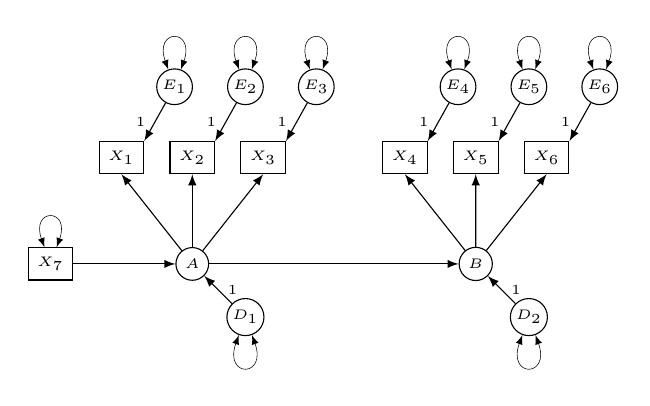
\begin{tikzpicture}[scale=0.9]
\node[draw, circle, inner sep=2] (l1) at (2,2) {\tiny{$A$}};
\node[draw] (o1) at (1,3.5) {\tiny{$X_1$}};
\node[draw] (o2) at (2,3.5) {\tiny{$X_2$}};
\node[draw] (o3) at (3,3.5) {\tiny{$X_3$}};
\node[draw, circle, inner sep=1] (l2) at (1.75,4.5) {\tiny{$E_1$}};
\node[draw, circle, inner sep=1] (l3) at (2.75,4.5) {\tiny{$E_2$}};
\node[draw, circle, inner sep=1] (l4) at (3.75,4.5) {\tiny{$E_3$}};
\node[draw, circle, inner sep=2] (l5) at (6,2) {\tiny{$B$}};
\node[draw] (o4) at (5,3.5) {\tiny{$X_4$}};
\node[draw] (o5) at (6,3.5) {\tiny{$X_5$}};
\node[draw] (o6) at (7,3.5) {\tiny{$X_6$}};
\node[draw, circle, inner sep=1] (l6) at (5.75,4.5) {\tiny{$E_4$}};
\node[draw, circle, inner sep=1] (l7) at (6.75,4.5) {\tiny{$E_5$}};
\node[draw, circle, inner sep=1] (l8) at (7.75,4.5) {\tiny{$E_6$}};
\node[draw] (o0) at (0,2) {\tiny{$X_7$}};
\node[draw, circle, inner sep=1] (l9) at (2.75,1.25) {\tiny{$D_1$}};
\node[draw, circle, inner sep=1] (l10) at (6.75,1.25) {\tiny{$D_2$}};
% Arrows
\draw [->, thin, >=latex] (l1)--(o1.south);
\draw [->, thin, >=latex] (l1)--(o2.south);
\draw [->, thin, >=latex] (l1)--(o3.south);
\draw [->, thin, >=latex] (l2)--(o1.north east) node[midway,left] {\tiny 1};
\draw [->, thin, >=latex] (l3)--(o2.north east) node[midway,left] {\tiny 1};
\draw [->, thin, >=latex] (l4)--(o3.north east) node[midway,left] {\tiny 1};
\draw [->, thin, >=latex] (l5)--(o4.south);
\draw [->, thin, >=latex] (l5)--(o5.south);
\draw [->, thin, >=latex] (l5)--(o6.south);
\draw [->, thin, >=latex] (l6)--(o4.north east) node[midway,left] {\tiny 1};
\draw [->, thin, >=latex] (l7)--(o5.north east) node[midway,left] {\tiny 1};
\draw [->, thin, >=latex] (l8)--(o6.north east) node[midway,left] {\tiny 1};
\draw [->, thin, >=latex] (l1)--(l5);
\draw [->, thin, >=latex] (o0)--(l1);
\draw [->, thin, >=latex] (l9)--(l1.south east) node[midway,right] {\tiny 1};
\draw [->, thin, >=latex] (l10)--(l5.south east) node[midway,right] {\tiny 1};
% Residuals:
\draw[<->, very thin, >=latex] (l2) to [out=70,in=110,looseness=9] (l2);
\draw[<->, very thin, >=latex] (l3) to [out=70,in=110,looseness=9] (l3);
\draw[<->, very thin, >=latex] (l4) to [out=70,in=110,looseness=9] (l4);
\draw[<->, very thin, >=latex] (l6) to [out=70,in=110,looseness=9] (l6);
\draw[<->, very thin, >=latex] (l7) to [out=70,in=110,looseness=9] (l7);
\draw[<->, very thin, >=latex] (l8) to [out=70,in=110,looseness=9] (l8);
\draw[<->, very thin, >=latex] (o0) to [out=70,in=110,looseness=9] (o0);
\draw[<->, very thin, >=latex] (l9) to [out=250,in=290,looseness=9] (l9);
\draw[<->, very thin, >=latex] (l10) to [out=250,in=290,looseness=9] (l10);
\end{tikzpicture}

\end{document}